% !TeX root = ../main.tex

\chapter{緒論}

本章為緒論,將簡述國內外電力需求狀況與傳統發電技術困境,並分別從電力系統發展、再生能源發展、電動汽車發展以及我國能源情勢等面相切入研究背景,最後說明本研究預期達到的目標以及章節組成架構。

\section{前言}

% 電力需求持續成長
能源是人類社會維持生存與文明發展所不可或缺的基礎資源,但隨著經濟發展與科技進步所延伸出的能源危機、空氣汙染與溫室效應等問題,儼然已是世界各國不得不面對的緊迫難題。長期以來,國內外的電力需求持續成長,圖 \ref{figure: Yearly Electricity Consumption in Taiwan} 為\uline{臺灣}地區年度用電數量 \cite{boe2021data},顯示自 $1999$ 年至 $2019$ 年間,\uline{臺灣}地區的年度用電數量由 $1,609$ 億度 ($160.9$ \si{\TWh}) 成長至 $2,666$ 億度 ($266.6$ \si{\TWh});於此同時,圖 \ref{figure: Yearly Electricity Consumption over World} 的世界各國年度用電數量 \cite{enerdata2020gesy} ,亦顯示世界各國的年度用電數量由 $126,050$ 億度 ($12,605$ \si{\TWh}) 成長至 $231,040$ 億度 ($23,104$ \si{\TWh}),其中又以我國在內的亞洲地區成長最為顯著。考量未來產業變遷、電動汽車普及等新增用電需求,我國經濟部預估在 $2021$ 年至 $2027$ 年間,\uline{臺灣}地區平均用電數量每年將成長約 $2.50\%$,年度用電數量將於 $2025$ 年達到 $3,091$ 億度 ($309.1$ \si{\TWh}) \cite{boe2021report}。

% 年度用電量統計數據
\begin{figure}[h]
  \centering
  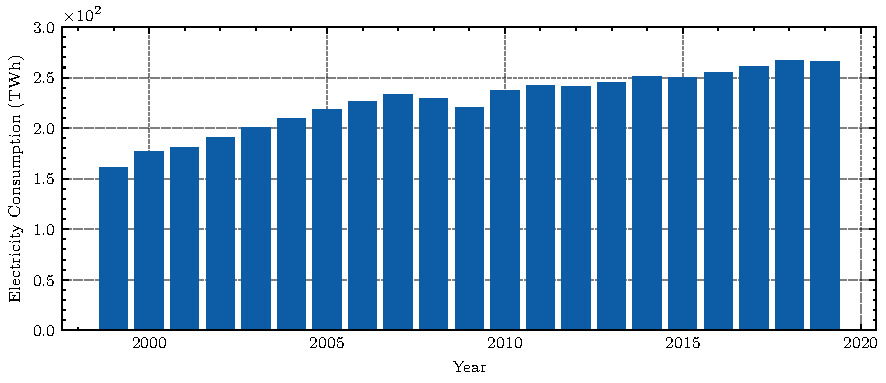
\includegraphics[width=\textwidth]{yearly-electricity-consumption-in-taiwan}
  \caption[\uline{臺灣}地區年度用電量]{\uline{臺灣}地區年度用電數量 \cite{boe2021data}}
  \label{figure: Yearly Electricity Consumption in Taiwan}
\end{figure}

\begin{figure}[h]
  \centering
  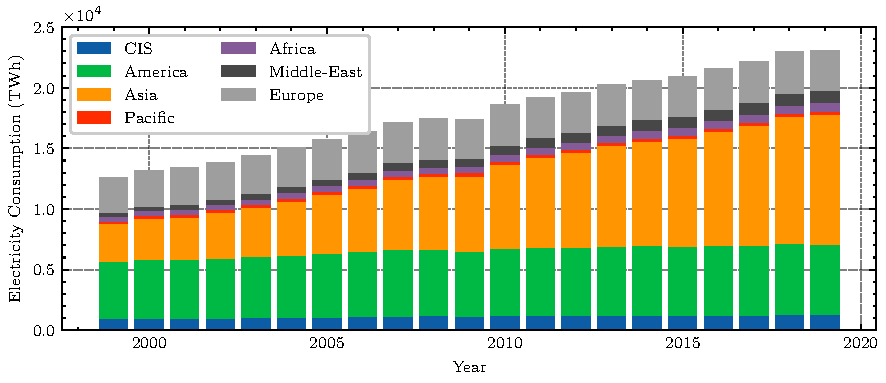
\includegraphics[width=\textwidth]{yearly-electricity-consumption-over-world}
  \caption[世界各地年度用電量]{世界各地年度用電數量 \cite{enerdata2020gesy}}
  \label{figure: Yearly Electricity Consumption over World}
\end{figure}

% 傳統發電佔比與缺點
目前世界各國的電力來源,主要以火力發電與核能發電為主,統計資料顯示,在 $2020$ 年時,火力發電與核能發電約佔全球總發電數量的 $70.92\%$ \cite{owid2020electricity},在\uline{臺灣}更佔總發電數量的 $93.40\%$ \cite{boe2021data}。其中火力發電需要大量開發燃煤、石油與天然氣等不可再生能源,也因此導致相關產業的溫室氣體排放量居高不下;而核能發電雖然有著較高的發電效率,並且幾乎沒有空氣汙染問題,但卻隱含安全隱憂,比如 $1986$ 年發生於俄羅斯的\uline{車諾比}事件 (Chernobyl disaster)、$1979$ 年發生於美國的\uline{三哩島}事件 (Three Mile Island accident) 與 $2011$ 年發生於日本的\uline{福島}第一核電廠事故 (Fukushima Daiichi nuclear disaster)。

% 虛擬電廠概念興起
民眾環保意識抬頭與核能發電安全隱憂的時空背景下,世界各國開始重新審視既有的能源產業與政策。於此同時,能夠充分利用再生能源並具有良好環境效益的分散式發電 (Distributed Generation, DG) 觀念,受到了越來越多的關注;為了降低將分散式電源併入既有電力系統所帶來的不穩定性,人們致力於發展能夠即時監控與調度分散式電源的智慧電網 (smart grid) 技術,以及可以在電網運作發生問題時即時斷開,藉此提升電力系統可靠度的微型電網 (micro grid) 技術,隨著資訊與電網技術的進步,也使虛擬電廠 (Virtual Power Plant, VPP) 概念應運而生。

\section{研究背景}

\subsection{電力系統發展}

% 電力系統定義:集中式電力系統 / 分散式電力系統
電力系統是指由發電系統、輸電系統與配電系統所組成的複雜系統,負責處理電力供給中依序會經歷的發電 (generating)、輸電 (transmission) 與配電 (distribution) 等過程 \cite{gonen2015electric}。根據電力系統中的發電系統規模,可以分為集中式電力系統 (centralized generated power system) 與分散式電力系統 (distributed generated power system)。在集中式發電系統中,電力的供給是火力、水力或核能等大型發電廠發電後,透過變電所提升電壓再經由電網輸送到用電端。而分散式電力系統,一般是由裝置容量較小的中小型發電設備所組成,分散地布置於用電端周圍 \cite{nissen2009high}。

% 臺灣供電系統架構
目前我國包含\uline{臺灣}本島、\uline{澎湖}、\uline{金門}與\uline{馬祖}在內之電力供應,由隸屬於中華民國經濟部的國營事業機構------\uline{臺灣}電力股份有限公司負責,其供電系統架構如圖 \ref{figure: Taiwan Power System Structure} 所示,圖中由火力、水力與核能發電廠產生的電力,需透過變壓器將電壓提升至超高壓 ($345$ \si{\kV}),再利用輸電線路輸送電力,然後經由超高壓變電所 ($161$ \si{\kV}) 與一次變電所 ($69$ \si{\kV})降壓後提供大型用戶用電,並透過配電變電所、二次變電所及配電系統再進行降壓,提供一般用戶使用 \cite{taipower2019supply}。

\begin{figure}[htbp]
  \centering
  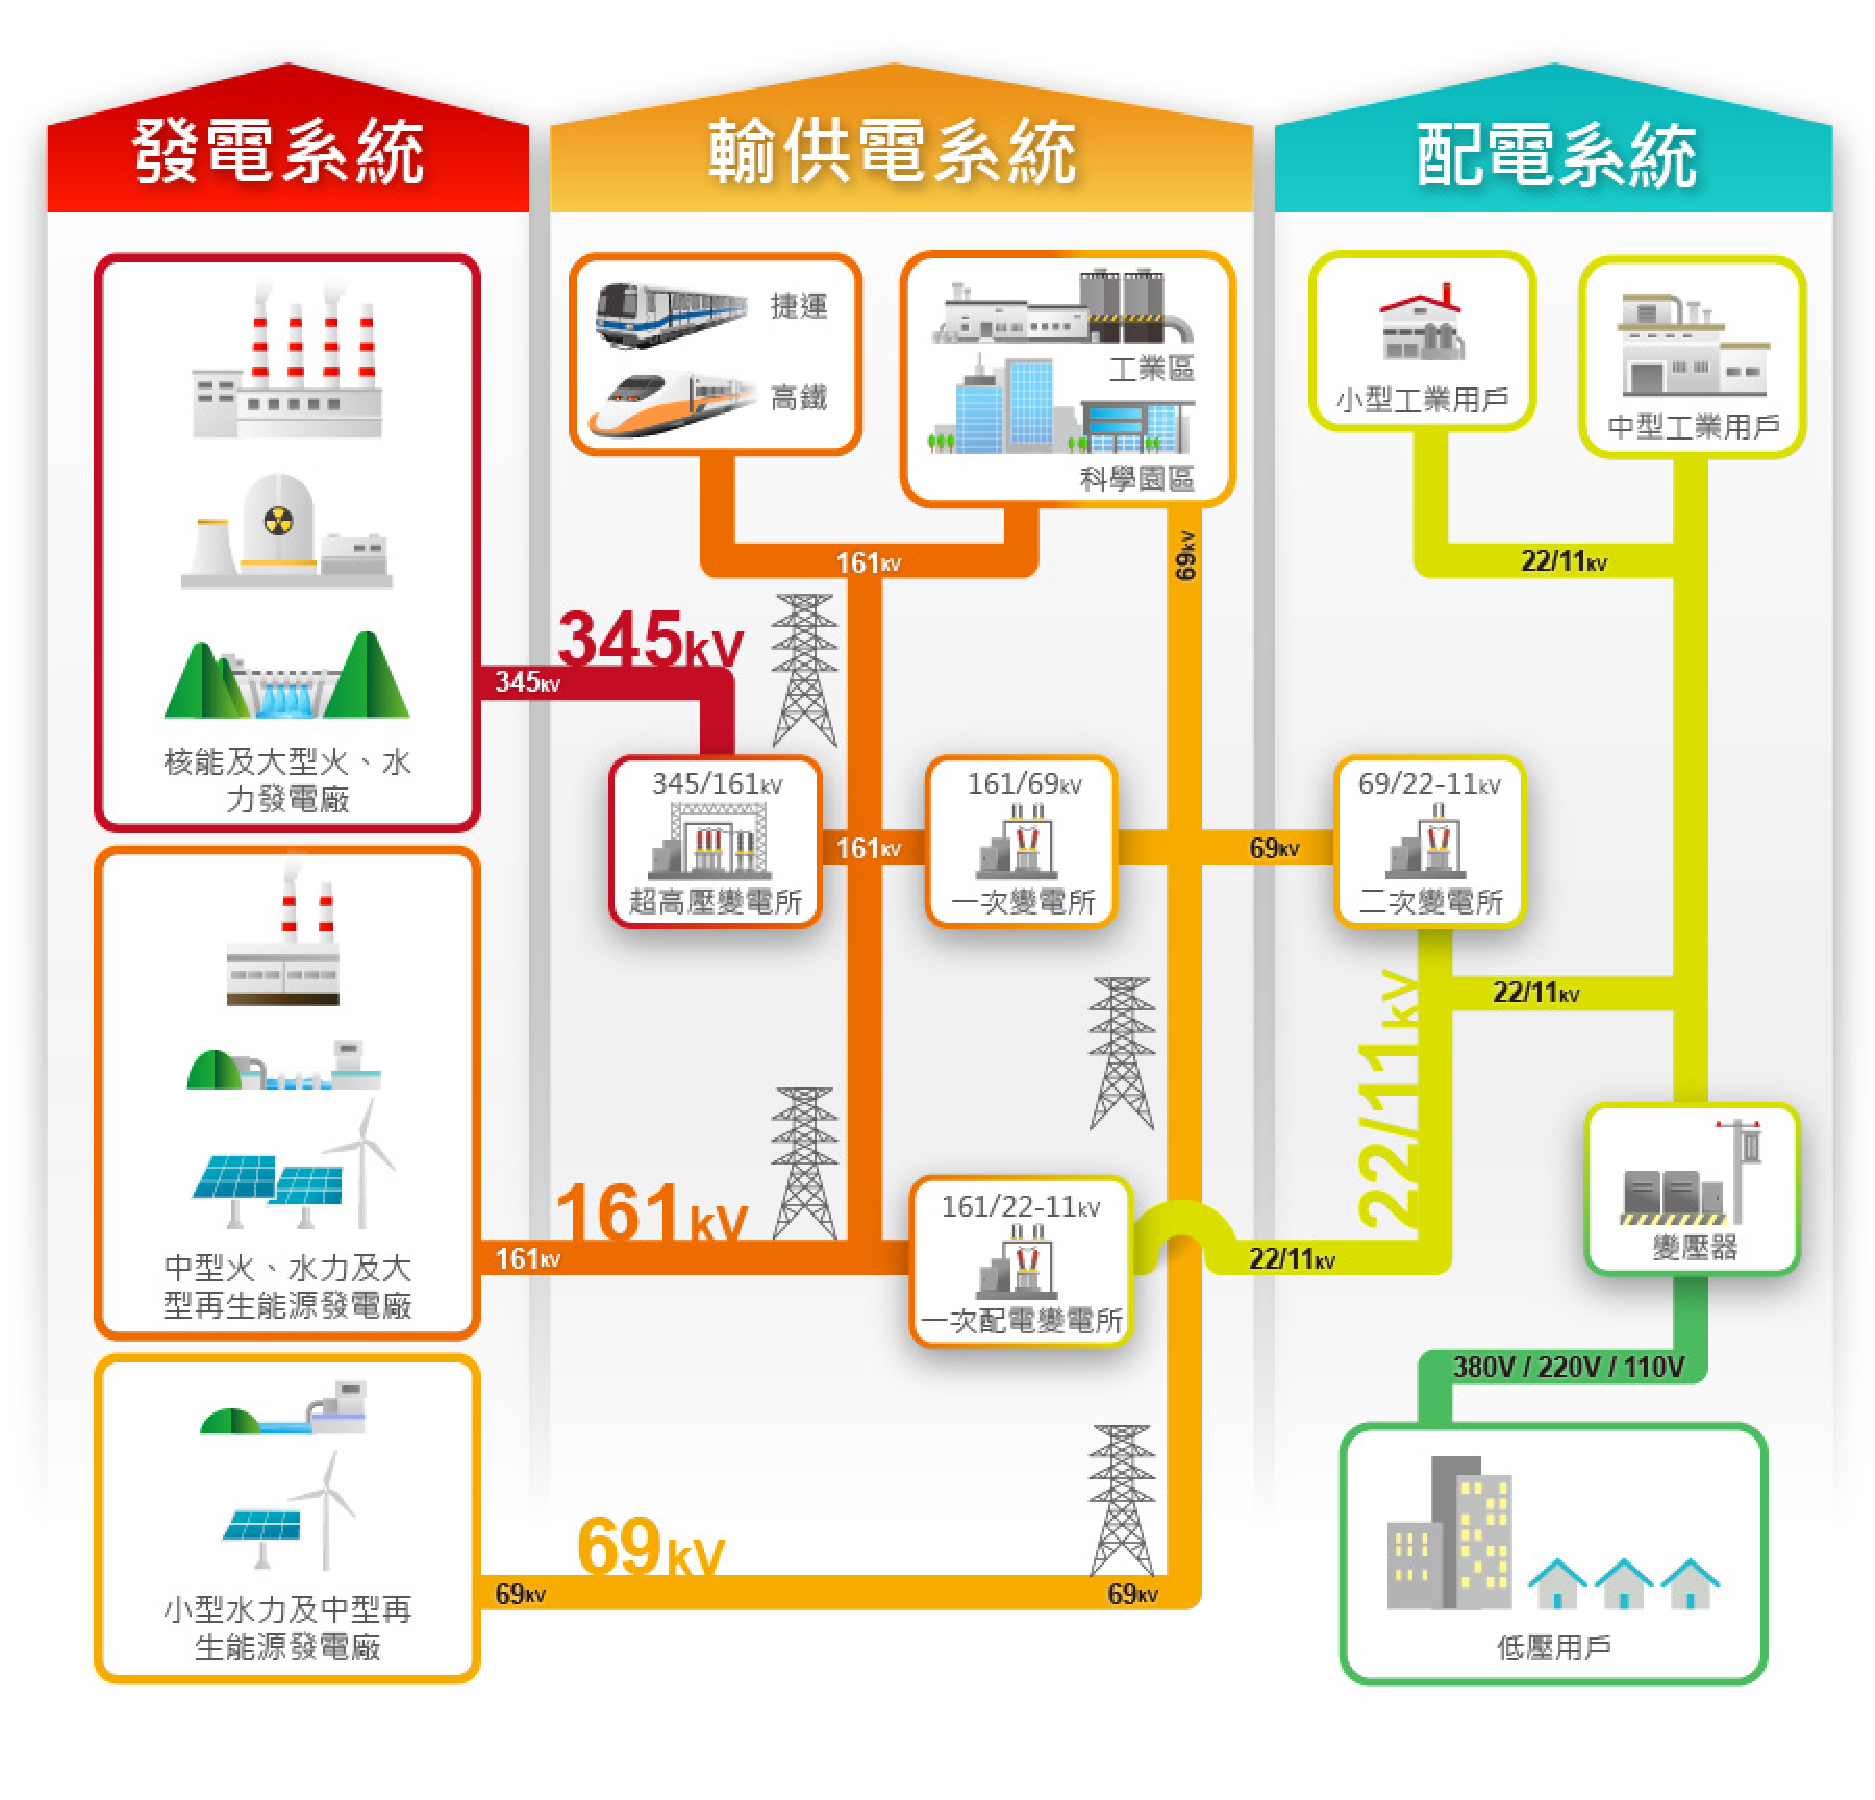
\includegraphics[width=0.75\textwidth]{Taiwan Power System Structure}
  \caption[臺灣電力股份有限公司供電系統架構]{臺灣電力股份有限公司供電系統架構 \cite{taipower2019supply}}
  \label{figure: Taiwan Power System Structure}
\end{figure}

% 傳統發電系統困境
現今世界各國的電力系統仍以傳統的集中式發電系統為主,雖然長期以來具有很好的規模經濟效益,然而隨著經濟與科技的發展,人們對於能源供給穩定性的要求日益提高,傳統集中式大型電網系統的缺陷也逐漸浮現。目前所面臨的問題,大致上可以歸納為以下幾點:

\begin{itemize}
  \item \textbf{發電機組集中建設,長距傳輸能量折損}:考量到建設成本,發電機組與用電用戶所在地通常距離遙遠,容易導致電力生產與分配不均,需要跨區輸電來解決電力不足問題,如此長距離的電力傳輸過程所累積的能量損失亦十分可觀。以\uline{臺灣}地區為例,輸電系統分為北、中、南三個地區,過往資料顯示在用電的尖峰季節,北部地區的電力仍需依靠中南部地區補足,而在過去十年間臺灣地區的電力線路損失率約為 $4\%$ \cite{boe2021data}。
  \item \textbf{局部故障影響整體,供電穩定備受考驗}:在輸配電網中,超過負載的高壓電纜將使得過載電流必須由附近的其他輸配電纜負責分攤,大量的電流回流可能導致輸配電纜超出負載而燒斷,最終故障擴散而導致大面積的停電效應。比如 $2003$ 年美加大停電、$2006$ 歐洲大停電、$2012$ 年印度大停電、$2018$ 日本\uline{北海道}大停電與 $2021$ 美國\uline{德州}大停電等大規模停電事件。
  \item \textbf{發電倚賴化石燃料,悖離能源永續目標}:燃煤、石油與天然氣等火力發電燃料屬於不可再生能源,在生產電力的過程中也伴隨著溫室氣體的排放,核能發電亦隱含安全隱憂。國際間越趨重視相關環境保護與資源永續問題,傳統集中式大型電網的主要發電方式勢必需要改善。
\end{itemize}

% 分散式發電、智慧電網、微型電網
由於上述集中式發電系統的種種問題,能夠有效利用再生能源的分散式發電系統越發受到重視,受限於裝置容量較小無法逕自取代大型電廠進行供電,分散式能源目前多採併入既有電網的形式,但再生能源本身具有的隨機性可能會阻礙電力系統的運行 \cite{guan2009research},為了儘量減少併網所引起的線路耗損與不可靠性,世界各國均致力於發展智慧電網與微型電網。智慧電網由電力系統與資訊系統所構成,藉由感測器即時監控電網系統行為,分析電力供給與需求後,再根據資訊即時調整電力系統狀態;微型電網可以視作一個小型的電力系統,整合多個中小型發電機組與電力用戶組成拓撲結構,可以透過切換連接模式或孤島模式,提升電力系統可靠度。除此之外,使用智慧電網與微型電網技術整合不同分散式能源的虛擬電廠亦受到各方重視,\uline{美國}、\uline{德國}、\uline{日本}、\uline{中國}與\uline{法國}等紛紛開始發展相關研究項目,盼能在解決電力調度與穩定運行問題的同時,打破傳統垂直壟斷的電力市場,建立競爭的市場機制。

\subsection{再生能源發展}

% 再生能源定義
再生能源 (renewable energy) 是指能夠持續不斷地從自然過程中獲取能量的資源,包括太陽能、風力、水力、地熱、生物燃料等;由於再生能源的獲得與使用過程中,所排放的汙染物相對較低,並且能降低對環境的危害性,因此又被稱作綠色能源 (green energy)。

表 \ref{table: Total 100-years CO2 Emissions from Different Energy Technologies} 為各類發電技術於生命週期內的碳排放量 \cite{jacobson2009review},使用二氧化碳當量 (carbon dioxide equivalent, CO2e) 作為測量碳足跡 (carbon footprints) 的標準單位,並以 $100$ 年排放量作為基準,資料顯示風力發電與太陽能發電的碳排放量,相較於其他發電技術都要來的少;然而再生能源所能帶來的益處遠不止於此,一份以美國\uline{加州}地區以量化工具衡量風力發電與太陽能發電的研究指出,若是提高太陽能與風力發電的裝置容量與發電數量,同時進行水資源管理,可以減少人們對於地下水的需求,進一步降低供水壓力與糧食危機 \cite{He2019}。

\begin{table}[htbp]
  \centering
  \caption[各類發電技術於生命週期內的碳排放量]{各類發電技術於生命週期內的碳排放量 \cite{jacobson2009review}}
  \begin{threeparttable}[t]
  \begin{tabular}{lccc}
    \toprule
    \textbf{能源技術} & \textbf{生命週期排放} \tnote{1} & \textbf{延遲機會成本} \tnote{2} & \textbf{人為熱量排放} \tnote{3} \\
    \midrule
    天然氣 & $179 \sim 405$ & $46 \sim 62$ & $0.61$ \\
    陸域風電 & $7.0 \sim 10.8$ & $0$ & $-1.7 \sim -0.7$ \\
    離岸風電 & $9 \sim 17$ & $0$ & $-1.7 \sim -0.7$ \\
    地熱發電 & $15.1 \sim 55.0$ & $14 \sim 21$ & 0 \\
    水力發電 & $17 \sim 22$ & $41 \sim 61$ & 0 \\
    海浪發電 & $21.7$ & $4 \sim 16$ & $0$ \\
    潮汐發電 & $10 \sim 20$ & $4 \sim 16$ & $0$ \\
    核能發電 & $9 \sim 70$ & $64 \sim 102$ & $1.6$ \\
    生物燃料 & $43 \sim 1730$ & $36 \sim 51$ & $3.4$ \\
    燃煤發電 & $230 \sim 935$ & $46 \sim 62$ & $1.5$ \\
    太陽能板 (屋頂) & $15 \sim 34$ & $-12 \sim -16$ & $-2.2$ \\
    太陽能板 (工業) & $10 \sim 29$ & $0$ & $-2.2$ \\
    聚光太陽能熱發電 & $8.5 \sim 24.3$ & $0$ & $-2.2$ \\
    \bottomrule
    & & & \hfill \si[per-mode=symbol]{\gram\text{-CO2e}\per{\kilo\watt\hour}}
  \end{tabular}
     \begin{tablenotes}
     \item[1] {\footnotesize 包括了建造、運轉與生產過程中所產生的碳排放}
     \item[2] {\footnotesize 建造與運營之間的時間延遲及壽命結束時翻新技術的額外停機時間}
     \item[3] {\footnotesize 包括燃燒或核反應釋放到空氣中的人為碳排放;太陽能發電技術透過將陽光轉換為電能來減少表面陽光,因此呈現為負值}
  \end{tablenotes}
  \end{threeparttable}%
  \label{table: Total 100-years CO2 Emissions from Different Energy Technologies}
\end{table}%

% 風機裝置容量
\begin{figure}[htbp]
  \centering
  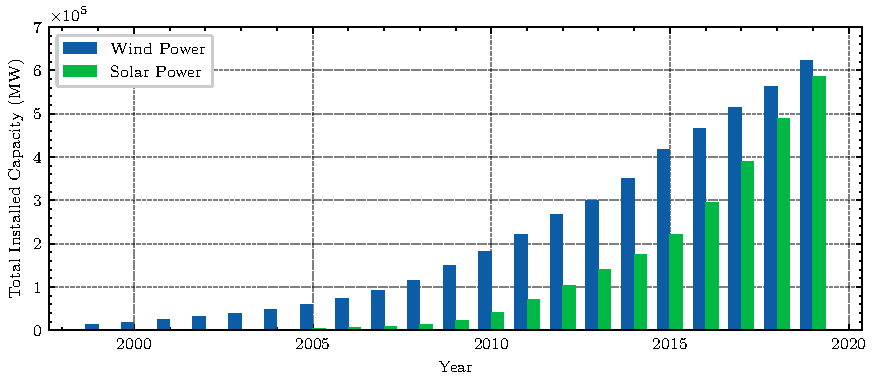
\includegraphics[width=\textwidth]{global-wind-and-solar-power-installation}
  \caption[全球風力與太陽能發電累積裝置容量]{全球風力與太陽能發電累積裝置容量 \cite{owid2020renewable}}
  \label{figure: Global Wind and Solar Power Installation}
\end{figure}

% 國際風力與太陽能發展
聯合國為了抑制持續嚴峻的全球暖化現象,於 $1997$ 年制定「\uline{京都}議定書」,規範工業國家未來的溫室氣體排放目標,各國此後逐漸將能源產業開發重心轉移至能夠減少碳足跡的核能發電與再生能源上。圖 \ref{figure: Global Wind and Solar Power Installation} 為 $1999$ 年至 $2019$ 年的全球風力發電與太陽能發電累積裝置容量 \cite{owid2020renewable},顯示全球的風力發電累計裝置容量從 $1999$ 年僅 $13,426$ 千瓩 ($13,426$ \si{\MW}),成長至 $2019$ 年的 $622,704$ 千瓩 ($622,704$ \si{\MW});而太陽能發電累計裝置容量則自 $1999$ 年僅 423 千瓩 ($423$ \si{\MW}),成長至 $2019$ 年的 $586,421$ 千瓩 ($586,421$ \si{\MW}),不難看出無論是風力發電亦或是太陽能發電皆發展迅速,足以彰顯各國落實減碳的決心

國際能源署 (International Energy Agency, IEA) 在 2021 年發布了一份關於全球如何在 2050 年達到淨零碳排的報告,說明如何在確保穩定能源供應的前提下,過渡到達成淨零碳排的目標,報告中提出了兼具成本效益與經濟生產的途徑,即是以風力發電和太陽能發電為基礎實現潔淨且有彈性的能源經濟 \cite{iea2021net}。近年來,受到招標競標與綠色憑證等市場機制影響,加上國際政策支持和建置成本降低,風力發電與太陽能發電等再生能源發展前景十分強勁,全球風能協會 (Global Wind Energy Council, GWEC) 預估到 $2024$ 年風力發電將再有約 $300,000$ 千瓩 ($300,000$ \si{\MW}) 的新增裝置容量 \cite{ohlenforst2019global},國際能源署則預估到 $2024$ 年時,太陽能發電的新增裝置容量將成長至 $600,000$ 千瓩 ($600,000$ \si{\MW}) \cite{iea2019report}。

\subsection{電動汽車發展}

% 電動汽車定義
電動車 (Electric Vehicle, EV) 是指具備單個或多個電動馬達,得以將電能轉換為動能來驅動的車輛。對於環境永續的議題而言,傳統依賴內燃機帶來動力的交通工具,在離開生產線之後,每單位里程的溫室氣體排放量就已經固定了下來;而電動汽車的溫室氣體排放量,卻能夠隨著能量來源越趨潔淨而逐年降低。近年來科技發展迅速,電動汽車電池的使用方式,除了過往由電網供電至電動汽車的 G2V (Grid to Vehicle) 模式,亦發展出了能夠反向由電動汽車輸電至電網的 V2G (Vehicle to Grid) 模式,因此電動汽車能夠在閒置或離峰時段作為電網調度的儲能設備,起到不同時段下電力資源調度的消峰填谷作用。

% 電動汽車成長
過去電動車難以普及的原因,就供給端而言,最大的問題在於生產成本居高不下;而就需求端來說,則是續航里程不高與充電方便性受限。然而隨著技術進步,不僅僅使得電動車續航里程得以提高,更使電池生產成本自 2010 年的每度電 $1,182$ 美元,下降至 $2020$ 年的每度電 $105$ 美元,生產成本已與燃油車相近。圖 \ref{figure: Global Electric Vehicles Stock} 為全球電動車累計數量,顯示在過去十年中電動汽車數量呈現穩定增長,於 2020 年時累計已超過 $1,126$ 萬輛電動汽車,預估將在 $2030$ 年成長至 $1.45 \sim 2.30$ 億輛電動汽車\footnote{此處的統計數字與預估數量包含油電混合車,但不包含兩輪或三輪的電動機車};除此之外,目前全球 $20$ 大汽車製造商中,已有 $18$ 家宣布增加電動汽車型號的製造數量,並訂定未來僅販售電動汽車的計畫 \cite{iea2021ev}。

% 風機裝置容量
\begin{figure}[htbp]
  \centering
  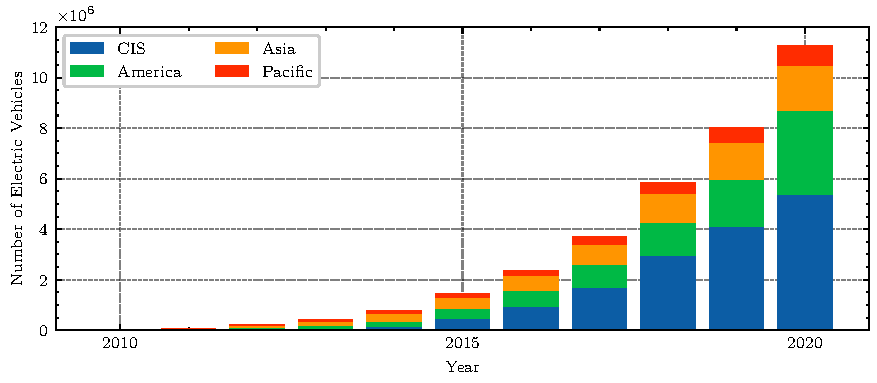
\includegraphics[width=\textwidth]{global-electric-vehicles-stock}
  \caption[全球電動車累計數量]{全球電動車累計數量 \cite{iea2021ev}}
  \label{figure: Global Electric Vehicles Stock}
\end{figure}

% 空氣汙染 -> 再生能源發展
值得一提的是,聯合國國際資源委員會 (International Resource Panel) 在 2016 年的產業報告指出,在燃煤佔比超過七成的國家推動電動汽車發展,會導致空氣汙染增加 \cite{hertwich2016green},而在 2019 年一份針對中國不同省份,了解電動車碳足跡在區域間變異性的研究,亦發現在燃煤發電佔有率較高的山東、河北等北方省份,電動汽車的碳足跡相較於燃煤汽車要來的高 \cite{wu2019assessing}。因此,單獨發展電動汽車並不能夠一勞永逸解決環境議題,如果未能同時提高綠色能源佔比,甚至可能會造成負面效果,隨著世界各國電動汽車產業的蓬勃發展,推動再生能源的進程更是刻不容緩。

\subsection{我國能源情勢}

\uline{臺灣}再生能源發展與我國政府為了因應「\uline{京都}議定書」所規範的溫室氣體減量標準有關,行政院於 1998 年召開的第一次全國能源會議,提出了以減碳為主要目標,鼓勵發展再生能源技術,首度將溫室氣體減量目標納入政策中。在 2008 年,行政院通過了《永續能源政策綱領》與《再生能源發展條例》,期望藉由政策規劃來改變能源架構,並將有限資源作有效的使用,兼顧能源安全、經濟發展與環境保護,以滿足未來世代發展的需要;在 2012  年,我國將智慧電網列入「國家節能減碳總計畫」中,致力於推動智慧電網技術,並實際推展至澎湖縣\uline{東吉島}、屏東縣\uline{林邊鄉}等處進行實域驗證;在 2015 年,通過了《溫室氣體減量及管理法》,明定國家溫室氣體長期減量目標,期望在 2050 年將溫室氣體排放量降低至 2005 年的 $50\%$ 以下。

% 臺灣政府雖在 2021 年 4 月 22 日世界地球日表態「支持 2050 淨零未來」,然而目前僅計劃在 2030 年減少 20% 碳排放,再生能源更只佔電力結構的 5.6%,發展龜步。邀請您加入推動改變的力量,透過分享文章訊息、支持能源轉型、要求政府制定足以對抗氣候危機的政策、加速發展再生能源,為您我與下一代打造一個永續、宜居、免於極端氣候威脅的地球家園。

% 我國為減少空氣汙染,行政院於 $2017$ 年通過的《空氣w汙染防制行動方案》中將分三階段推動全台電動車化,目標於 $2040$ 年達到新售汽機車全面自動化。近年來在政府補貼政策激勵下,電動汽機車逐漸受到民眾認可與青睞,電動汽機車佔新增汽機車掛牌數量逐年上升。

% 千架海陸風力機 / 陽光屋頂百萬座
為落實\uline{臺灣}環境永續,我國經濟部於 2012 年,針對風力發電與太陽能發電推動相關計畫,規劃於 2030 年達成「陽光屋頂百萬座 、千架海陸風力機」兩項願景。考量國際趨勢與民意聲浪,我國於 2016 年政黨輪替後,加速興建第三座天然氣接收站,擬定在 2025 年全面廢除核能發電並降低燃煤發電比例,達成「非核家園」的目標;為推度臺灣產業轉型,我國政府亦於 2018 年提出包含「綠能科技」產業在內的 $5+2$ 產業創新計畫,積極推動「太陽光電兩年推動計畫」、「綠能屋頂全民參與」、「風力發電四年推動計畫」、「智慧電表示範建置」、「沙崙智慧綠能科學城」等計畫,希望結合國內需求發展相關能源產業,引進國內外投資的同時增加國內需求與就業機會。為了補足廢除核能發所出現的能源缺口,立法院於 2019 年通過《再生能源發展條例》修正案,更加積極推動再生能源發展,設立 2025 年達成再生能源發電數量佔總發電數量 $20\%$ 的目標。

表 \ref{table: Renewable Energy Device Ratio in Taiwan} 為 2008 年《再生能源發展條例》通過後,我國再生能源裝置容量與發電數量之狀況 \cite{boe2021data},顯示我國再生能源發展步調雖穩健但緩慢,以此成長趨勢要在 $2025$ 年達到再生能源發電數量佔比 $20\%$ 的目標,尚有好幾許哩路要走。

\begin{table}[htp]
  \centering
  \caption[臺灣地區再生能源裝置容量與發電數量]{臺灣地區再生能源裝置容量與發電數量 \cite{boe2021data}}
  \begin{tabular}{crrrr}
    \toprule
    \textbf{年度} & \textbf{裝置容量} & \textbf{裝置容量佔比} & \textbf{發電數量} & \textbf{發電數量佔比} \\
                  & (\si{\MW})        & (\%)                  & (\si{GWh})        & (\%)                  \\
    \midrule
    $2019$        & $7,795$           & $13.9$ \%             & $15,360$          & $5.6$ \%              \\
    $2018$        & $6,246$           & $11.9$ \%             & $12,634$          & $4.6$ \%              \\
    $2017$        & $5,259$           & $10.7$ \%             & $12,390$          & $4.6$ \%              \\
    $2016$        & $4,726$           & $ 9.5$ \%             & $12,753$          & $4.8$ \%              \\
    $2015$        & $4,330$           & $ 8.9$ \%             & $10,501$          & $4.1$ \%              \\
    $2014$        & $4,065$           & $ 8.4$ \%             & $ 9,944$          & $3.8$ \%              \\
    $2013$        & $3,816$           & $ 7.8$ \%             & $10,864$          & $4.3$ \%              \\
    $2012$        & $3,594$           & $ 7.4$ \%             & $10,684$          & $4.3$ \%              \\
    $2011$        & $3,399$           & $ 7.0$ \%             & $ 8,995$          & $3.6$ \%              \\
    $2010$        & $3,197$           & $ 6.5$ \%             & $ 8,642$          & $3.5$ \%              \\
    $2009$        & $3,030$           & $ 6.3$ \%             & $ 7,808$          & $3.4$ \%              \\
    \bottomrule
  \end{tabular}
  \label{table: Renewable Energy Device Ratio in Taiwan}
\end{table}

除此之外,我國行政院於 2017 年完成《電業法》修正,開放再生能源自由交易,未來\uline{臺灣}的電力市場將採躉購制度與自由市場雙軌運作,落實電業自由化 (electricity liberalization) 以推動我國綠色產業發展;負責營運電力交易平台的電力交易中心於 2021 年 7 月 1 日揭牌啟用,劃下我國電力產業轉型的重要里程碑,平台首先推出有別於直接購買電力資源的「日前輔助服務市場」的交易制度,鼓勵民間將分散式電力資源投入平台參與電力市場交易以維持電網穩定。

% 為了由根本解決傳統大型電網所衍生出的種種問題,並邁向永續能源發展之最終目標, 智慧電網與微電網的建設、再生能源的開發以及政府政策的訂定均為不可忽略的發展方向。 因此,除了仰賴科技發展與設備的進步外,本研究希望能藉由區域性能源供需數據與電網 配電控制策略的整合提高能源使用效率,並透過電力系統設備規劃建立階段性任務,以確 保電力系統能逐步朝能源永續的目標邁進。

% 目前,無論是在確保能源穩定供應、發展潔淨能源或是提高能源使用效率等方面,均 有許多不同領域的學者致力於相關的研究,但並沒有一套有系統的方法將各研究方向進行 整合;此外,充分利用自然資源的再生能源發電方式雖然永續,但不同的自然資源會因為 地域的不同而有不同特性,再加上自然現象的變動常導致電力無法穩定供應與預測。因此, 一個完善的永續能源發展策略需要依照各地區不同的自然資源與環境特性進行規劃,以達到整體電力系統之階段性目標,引領電力系統朝能源永續邁進。

% 綜合以上,我國發展再生能源是十分可行的,但目前尚在推廣階段,而政府 所規劃、未來預計建置的裝置容量僅為期望,要實際實踐還須政府積極推廣並提 高民間參與意願。此外,以客觀學術方式檢視目前政府所規劃的再生能源發展目 標能否順利達成亦是重要議題之一,因此本研究擬應用時間序列分析方法,根據 我國歷年裝置容量數據及目前所規劃之發電能源裝置容量來建立火力及汽電共生 裝置容量預測模型,並利用預測結果配合不同達成率的「千架海陸風力機」、「陽 光屋頂百萬座」及「地面型 PV 系統可用地」等計畫作情境分析模擬,檢視我國政 府規劃 2025 年再生能源目標能否順利完成與非核家園的可能,以及對用電需求與 環境的影響。

% 電力市場自由化

\section{研究動機}

\uline{臺灣}地區地狹人稠,能源高度仰賴進口,未來核能電廠陸續除役後所造成的電力缺口,不論對民生或是經濟發展,都是一個迫切需要解決的問題。在國際情勢與民意傾向下,額外增設火力電廠必然不是首要選項,而智慧電網與微型電網的發展,讓虛擬電廠概念得以落地應用,加上電力市場自由化的到來,吸引系統營運商投資並且採用虛擬電廠,或許是一個可以嘗試的辦法。

在蒐集文獻的過程中,發現國內關於虛擬電廠的相關研究並不多,並且大多以商業模式分析為主,尚缺少一套客觀評估虛擬電廠收益的工具。考慮我國目前風力發電與太陽光電的累計裝置容量差異不大,且風力發電在相近容量裝置下,比起太陽光電具有更高的發電效率,加上國內外電動汽車產業成長趨勢顯著,本研究希望能結合風力發電與電動汽車,以車輛對電網 (Vehicle-to-Grid, V2G) 概念為基礎,構建虛擬電廠收益模型,並根據不同時段下的時間電價調度電力供需來最佳化虛擬電廠收益,以供電廠業者作為收益評估及決策之參考。

\section{研究目的}

綜合上述研究背景與研究動機,本文的研究目的條列如下:

\begin{enumerate}[label = (\arabic*), itemsep=4pt, parsep=4pt, topsep=0pt, partopsep=0pt]
  \item 了解虛擬電廠概念,整理建構收益模型所需的資料與流程;
  \item 依據資料蒐集結果,建構一套整合風力電場與電動汽車的虛擬電廠收益模型;
  \item 針對收益模型建構過程中的困難與不足之處,提出方法、進行改善;
  \item 透過案例分析,探討在不同假設情境下虛擬電廠之收益狀況。
\end{enumerate}

本文旨在建構一套分析流程,用以計算虛擬電廠中在整合風力電場與電動汽車下的收益,期望能對今後相關政策與投資評估有所助益。

% 本文擬採用虛擬電廠概念整合近年來成長趨勢顯著的電動汽車作為機動性儲能設備,使再生能源得以透過能量儲存緩衝本身的隨機性與間歇性,以短期風速預測電量為基礎,建構虛擬電廠參與電力市場的收益分析模型,並使用模型預測控制方法 (Model Predictive Control, MPC) 在有限時域內根據過去狀態進行即時性調度,期望能對今後評估虛擬電廠收益有所助益。

\section{本文架構}

本文共分六章,整體架構如圖 \ref{figure: Thesis Organization} 所示。各章內容分述如下:第一章為緒論,針對論文研究背景、研究動機與研究目的進行說明;第二章為文獻回顧,介紹本文研究內容所涉及的領域,並將蒐集到的國內外相關文獻進行統整與探討;第三章為研究方法,簡述研究流程及方法原理,做為日後驗證結果有效性的基礎;第四章為模型建構,說明本文依據前提文獻及研究方法所建構的收益模型及其建構方式;第五章為案例分析,示範分析過程並探討不同假設情境下的虛擬電廠收益狀況;第六章為結論與建議,依本研究所得到結果進行總結,最後補充說明研究限制並對未來可行的研究方向提出建議。

% [Figure] 論文架構
\begin{figure}[htbp]
  \centering
  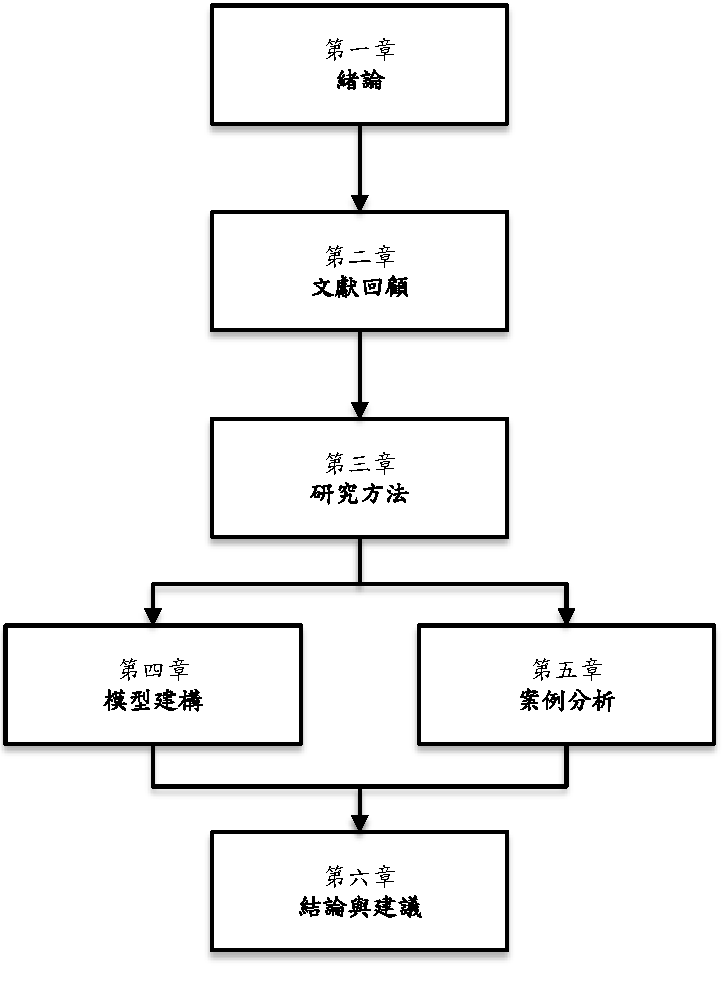
\includegraphics{thesis-organization}
  \caption[論文架構]{論文架構}
  \label{figure: Thesis Organization}
\end{figure}